\documentclass[12pt,a4paper,onecolumn]{article}

%%%%%%%%%%%%%%%%%%%%%%%%%%%%%%%%%%%
%          				PACKAGES  				              %
%%%%%%%%%%%%%%%%%%%%%%%%%%%%%%%%%%%

%\usepackage[margin=1in]{geometry}
\usepackage[top=2cm, bottom=2.5cm, left=2.5cm, right=2.5cm]{geometry}

\usepackage{authblk}
\usepackage[latin1]{inputenc}
\usepackage{amsfonts}
\usepackage{graphicx,color}
\usepackage{amsmath}
\usepackage{amssymb}
\usepackage[table]{xcolor}
\usepackage{setspace}
\usepackage{booktabs}
\usepackage{dcolumn}
\usepackage{rotating}
\usepackage{color,soul}
\usepackage{threeparttable}
\usepackage[capposition=top]{floatrow}
\usepackage[labelsep=period]{caption}

\usepackage{subcaption}
\usepackage{lscape}
\usepackage{pdflscape}
\usepackage{multicol}
\usepackage[bottom]{footmisc}
\setlength\footnotemargin{5pt}
\usepackage{longtable} %for long tables

\usepackage{enumerate}
\usepackage{units}  %nicefraction
\usepackage{placeins}
\usepackage{booktabs,multirow}
%% BibTeX settings
\usepackage{natbib}
\bibliographystyle{apalike}
%\bibliographystyle{unsrtnat}
\bibpunct{(}{)}{,}{a}{,}{,}

% Codificación y tipografías correctas
\usepackage[utf8]{inputenc}   % permite escribir áéíóúñ directamente
\usepackage[T1]{fontenc}      % hyphenation y copiado correcto con 
\usepackage{lmodern}          % fuentes con T1 (Latin Modern)

\usepackage{enumitem} % listas sin sangría extra

%% paragraph formatting
\renewcommand{\baselinestretch}{1}


% Defines columns for tables
\usepackage{array}
\newcolumntype{L}[1]{>{\raggedright\let\newline\\\arraybackslash\hspace{0pt}}m{#1}}
\newcolumntype{C}[1]{>{\centering\let\newline\\\arraybackslash\hspace{0pt}}m{#1}}
\newcolumntype{R}[1]{>{\raggedleft\let\newline\\\arraybackslash\hspace{0pt}}m{#1}}

\usepackage{comment} %to comment entire sections

\usepackage{xfrac} %sideways fractions


\usepackage{bbold} %for indicators

\setcounter{secnumdepth}{6}  %To get paragraphs referenced 

\usepackage{titlesec} %subsection smaller
\titleformat*{\subsection}{\normalsize \bfseries} %subsection smaller
%\usepackage[raggedright]{titlesec} % for sections does not hyphen words


\usepackage[colorlinks=true,linkcolor=black,urlcolor=blue,citecolor=blue]{hyperref}  %Load last
%% markup commands for code/software
\let\code=\texttt
\let\pkg=\textbf
\let\proglang=\textsf
\newcommand{\file}[1]{`\code{#1}'}
\newcommand{\email}[1]{\href{mailto:#1}{\normalfont\texttt{#1}}}
\urlstyle{same}
%%%

\usepackage{makecell}

\usepackage{graphicx}

%%%%%%%%%%%%%%%%%%%%%%%%%%%%%%%%%%%
%     			TITLE, AUTHORS AND DATE    			  %
%%%%%%%%%%%%%%%%%%%%%%%%%%%%%%%%%%%

\title{\textbf{Understanding and Predicting Wages: Evidence from Bogot\'a}}

%\large {Machine Learning and Big Data, School of Economics, Universidad de los Andes}

\author{Juan Jos\'e Rojas, Francisco Soler, Jes\'us Yancy \& Juan Otalora}

\date{}

%%%%%%%%%%%%%%%%%%%%%%%%%%%%%%%%%%%
%          				  DOCUMENT       					      %
%%%%%%%%%%%%%%%%%%%%%%%%%%%%%%%%%%%

\begin{document}
\maketitle
\thispagestyle{empty}

\begin{center}
\texttt{Link to the GitHub repository: \url{https://github.com/jrconstain/PS1_Group4}}
\end{center}

\section{Introduction}

%%% Intructions: The introduction states the problem and any antecedents. It briefly describes the data and its suitability to address the problem set question. It contains a preview of the results and main takeaways. Keep this section up to 5 paragraphs.

Colombia has long struggled with insufficient tax revenue: the country consistently collects less and spends more than what its income level would predict \citep{Fergusson2022}. A significant portion of this gap stems from tax evasion, estimated at 8.6\% of GDP, of which 1.1\% corresponds to evasion in personal income taxes \citep{Lora2021a, Lora2021b}. Among these, labor income underreporting --though relatively modest-- still accounts for nearly 1.2 trillion Colombian pesos in lost revenue annually\footnote{This figure is obtained by applying the 0.07\% of GDP that \citet{Lora2021a} estimate as efficiently recoverable from labor income underreporting to the official 2024 GDP estimate for Colombia (COP 1,706.4 trillion) published by \citep{DANE2025a}}, equivalent to about twice the GDP of Guain\'ia and more than double that of Vaup\'es \citep{DANE2025a}. This paper addresses two main objectives: first, to explore the determinants of labor earnings by examining how individual characteristics--particularly age and gender--shape wage outcomes; and second, to develop predictive models that can identify potential underreporting in tax filings, contributing to the broader goal of reducing evasion.

Our analysis draws on data from the 2018 GEIH survey for Bogot\'a \citep{DANE2025b}. From an initial sample of 32,177 individuals, we restrict our focus to salaried workers aged 18 and over, excluding the self-employed and unpaid family workers. This yields a final study sample of 9,892 individuals. We concentrate on wages rather than total income, as salaries tend to be more stable and more strongly correlated with observable individual characteristics. This focus serves both our analytical and predictive goals: it enables precise identification of wage determinants while also providing a robust foundation for models aimed at detecting underreporting among formal employees.

The first set of our empirical results highlights two key patterns. First, the estimated age-wage profile follows a concave, parabolic shape with a peak around age 45, consistent with standard human capital theory. Second, the examination of the gender-earnings gap reveals a more nuanced picture than the 4.7\% difference of the unconditional model initially suggests. When controlling for individual characteristics such as education and age, the gap widens to 13\%, suggesting that the initial figure understates the disparity--partly because women in the sample are, on average, slightly more educated. Adding controls for firm characteristics (formality, sector, size) reduces the gap to 10\%, and further incorporating occupation fixed effects lowers it to 8.4\%. Even so, this final gap remains nearly twice the raw estimate, reflecting a mix of selection and discrimination effects that continues to shape gendered labor market outcomes.

Beyond the causal analysis, our predictive exercises demonstrate that wage outcomes can be forecast with reasonable accuracy using relatively parsimonious models. Across multiple specifications, models enriched with nonlinear terms for age and socioeconomic status consistently delivered the lowest prediction errors. In particular, the specification labeled Additional 2 achieved the best performance, with a Root Mean Square Error (RMSE) of 0.45, a result that proved robust under both K-fold and Leave-One-Out Cross-Validation. These findings suggest that predictive models can complement traditional econometric approaches by identifying patterns in the data that flag anomalous observations and, by extension, potential cases of underreporting in income declarations.

Taken together, our findings contribute to both the explanatory and predictive understanding of wage determination in Colombia. The evidence highlights how age and gender shape earnings, how firm and occupational sorting mediate the gender gap, and how predictive models can improve the detection of underreporting in labor income. The remainder of the paper is organized as follows. Section 2 describes the data and variable construction. Section 3 presents the econometric analysis of the age-wage profile, and Section 4 analyzes the gender-earnings gap. Section 5 develops the predictive models and evaluates their performance to close our excercise.

\section{Data}

We base our exercise on a dataset\footnote{Assembled by Professor Manuel Fern\'andez and made accessible via the website of Professor Ignacio Sarmiento, Universidad de los Andes. Publicly available at: \url{https://ignaciosarmiento.github.io/GEIH2018_sample/}. Importantly, no restrictions (such as a \texttt{robots.txt} file) prevented this collection.} extracted through a scraping routine to collect all 32,177 observations of individuals surveyed in Bogot\'a for the 2018 GEIH (\textit{Gran Encuesta Integrada de Hogares}). Conducted by DANE since 2006, the GEIH is Colombia's main source of labor statistics, covering employment, earnings, demographics, and income sources nationwide \citep{Banrep2025, DANE2025b}. From this universe, we restrict the sample to wage earners aged 18 and above, excluding the self-employed and unpaid family workers ($N=9{,}892$). Because the GEIH asks respondents about the number of hours worked during the previous week, values reported may reflect atypical events. We trimmed the top and bottom one percent of the distribution to account for these, excluding 192 cases. This yields our final analytic sample of $N=9{,}700$. We focus on labor income as a more stable outcome largely driven by individual characteristics such as age and education, in contrast to entrepreneurial or informal gains more prone to be affected by external, non-observable factors. 

To enrich our analysis, we constructed two additional variables. First, we derived \textit{years of education} from the GEIH questions \texttt{p6210} (highest level attained) and \texttt{p6210s1} (years completed), by summing the years required to get to the highest level attained and years reported as completed within that level. Second, following \citep{Fernandez2018}, we computed a measure of potential \textit{experience} as \ensuremath{\textit{age} - \textit{years of education} - 6}. These transformations allow us to approximate human capital more accurately across individuals.

Table~\hyperref[tab:ind_job_chars]{\ref{tab:ind_job_chars}} presents the descriptive statistics for the main variables included in our analysis. The average individual in the sample is 36.2 years old with 18.4 years of potential experience, showing little variation between men and women. Notably, women exhibit slightly higher educational attainment than men: they report an average of 12.2 years of education versus 11.5 for men, and their maximum educational level reached is also higher (6.20 vs. 6.01 on a seven-point scale). In contrast, labor outcomes show that men earn more on average, both monthly (COP 1,836,380 vs. COP 1,676,747) and hourly (COP 8,945 vs. COP 8,659), and also work more hours per week (49.9 vs. 46.6). Differences in employment structure are also apparent: a greater share of men are formally employed (78.9\% vs. 76.2\%), men are less likely to work in small firms (18.5\% vs. 25.5\%), and they tend to be employed in private firms (93.8\% vs. 83.8\%) and in slightly larger organizations on average (firm size 4.06 vs. 3.82).



\begin{table}[h!]
\caption{Individual and job characteristics: overall and by sex.}
\label{tab:ind_job_chars}
\centering
\resizebox{\textwidth}{!}{%
\begin{threeparttable}
\begin{tabular}{lccc}
\toprule
 & All (N=9{,}700) & Men (N=4{,}875) & Women (N=4{,}825) \\
\midrule
\multicolumn{4}{l}{\textbf{Panel A. Individual characteristics}} \\
Age (years) 
  & \makecell{36.232 \\ (11.986)}
  & \makecell{35.955 \\ (12.147)}
  & \makecell{36.513 \\ (11.815)} \\
Experience (years) 
  & \makecell{18.373 \\ (13.352)}
  & \makecell{18.429 \\ (13.360)}
  & \makecell{18.316 \\ (13.345)} \\
Socioeconomic level (1--6) 
  & \makecell{2.508 \\ (0.976)}
  & \makecell{2.438 \\ (0.949)}
  & \makecell{2.579 \\ (0.998)} \\
Maximum educational attainment\tnote{a}  (1--7)
  & \makecell{6.104 \\ (1.100)}
  & \makecell{6.013 \\ (1.115)}
  & \makecell{6.196 \\ (1.077)} \\
Years of education 
  & \makecell{11.866 \\ (3.999)}
  & \makecell{11.530 \\ (4.010)}
  & \makecell{12.206 \\ (3.959)} \\
\addlinespace[6pt]

\multicolumn{4}{l}{\textbf{Panel B. Earnings \& work hours}} \\
Labor income (monthly, COP)  
  & \makecell{1{,}756{,}975 \\ (2{,}412{,}230)}  
  & \makecell{1{,}836{,}380 \\ (2{,}493{,}475)}  
  & \makecell{1{,}676{,}747 \\ (2{,}324{,}769)} \\
Hourly labor income (COP/hour)  
  & \makecell{8{,}803 \\ (12{,}563)}  
  & \makecell{8{,}945 \\ (12{,}728)}  
  & \makecell{8{,}659 \\ (12{,}393)} \\
Total hours worked (week)  
  & \makecell{48.274 \\ (10.522)}  
  & \makecell{49.949 \\ (10.391)}  
  & \makecell{46.582 \\ (10.382)} \\
  \addlinespace[6pt]

\multicolumn{4}{l}{\textbf{Panel C. Employment structure (\%)}} \\
 \addlinespace[6pt]
Formal employment & 77.6 & 78.9 & 76.2 \\
\addlinespace[4pt]
Small firm ($\leq$5 employees) & 22.0 & 18.5 & 25.5 \\
\addlinespace[4pt]
Private employees & 88.8 & 93.8 & 83.8 \\
Firm size\tnote{b} & \makecell{3.94 \\ (1.32)} & \makecell{4.06 \\ (1.18)} & \makecell{3.82 \\ (1.44)} \\


  
\bottomrule
\end{tabular}

\begin{flushleft}\footnotesize
\textit{Notes:} Each numeric cell reports the \textit{Mean} on the first line and the \textit{Standard Deviation} (in parentheses) on the second line. Monetary values in Colombian pesos (COP). \textit{(a)} Firm size is an ordinal scale; higher values indicate larger firms. \textit{(b)} Maximum educational attainment ranges from 1 to 7 (with 6 = complete secondary, 11 years; 7 = tertiary). One observation is missing in this variable for the overall sample (All: $N=9{,}699$).
\end{flushleft}
\end{threeparttable}
}
\end{table}



\section{Age-wage profile}

To better understand the determinants of wages, we begin by examining the age-wage profile--a core building block of human-capital models since \citet{Mincer1974}--which captures how average earnings vary with an individual's age \citep{Startz2014}. This profile typically follows an inverted U-shape, with wages increasing until peaking in the early 50s, and then gradually declining as retirement nears. 
We estimate the following quadratic Mincerian specification, a standard reduced-form approach that captures the life-cycle wage pattern and allows identification of the turning point:

\begin{equation}
\log(w) \;=\; \beta_1 \;+\; \beta_2\,\text{Age} \;+\; \beta_3\,\text{Age}^2 \;+\; u,
\end{equation}

where $w$ denotes hourly wages, and $\beta_2 > 0$ and $\beta_3 < 0$ under the canonical concave profile.

\autoref{tab:agewage} show the results of our estimation. Both age coefficients exhibit the expected signs, implying a concave life-cycle profile consistent with human-capital accumulation and job-ladder mechanisms \citep{Mincer1974,Card1999}. The point estimates (0.069 on age; $-0.001$ on age$^2$) imply that hourly wages increase with age but at a diminishing marginal rate, a pattern prevalent across labor markets and cohorts \citep{MurphyWelch1990,LagakosEtAl2018}. As expected in a cross-sectional setting, the explanatory power of the model is modest ($R^2=0.047$; residual s.e.\ $=0.705$ log points). The remaining dispersion likely reflects variation in factors such as education, occupation, firm characteristics, and match quality-determinants emphasized in both empirical and structural literatures \citep{HeckmanLochnerTodd2006}.

% Table created by stargazer v.5.2.3
\begin{table}[!htbp] \centering 
  \caption{Unconditional Age--Wage Profile regression.} 
  \label{tab:agewage} 
\begin{tabular}{@{\extracolsep{5pt}}lc} 
\\[-1.8ex]\hline 
\hline \\[-1.8ex] 
 & \multicolumn{1}{c}{\textit{Dependent variable:}} \\ 
\cline{2-2} 
\\[-1.8ex] & Log Hourly Wage \\ 
\hline \\[-1.8ex] 
 Age & 0.069$^{***}$ \\ 
  & (0.004) \\ 
  & \\ 
 Age$^{2}$ & $-$0.001$^{***}$ \\ 
  & (0.00004) \\ 
  & \\ 
 Constant & 7.339$^{***}$ \\ 
  & (0.068) \\ 
  & \\ 
\hline \\[-1.8ex] 
Observations & 9,700 \\ 
R$^{2}$ & 0.047 \\ 
Adjusted R$^{2}$ & 0.047 \\ 
Residual Std. Error & 0.705 (df = 9697) \\ 
F Statistic & 239.598$^{***}$ (df = 2; 9697) \\ 
\hline 
\hline \\[-1.8ex] 
\textit{Note:}  & \multicolumn{1}{r}{$^{*}$p$<$0.1; $^{**}$p$<$0.05; $^{***}$p$<$0.01} \\ 
\end{tabular} 
\end{table} 

\autoref{fig:agecurve1} displays the estimated age--wage trajectory for the full sample of 9{,}700 workers (men and women combined), revealing a smooth concave pattern. Under the quadratic model, the turning point is given by:
\[
a^\ast \;=\; -\frac{\widehat{\beta}_2}{2\,\widehat{\beta}_3},
\]
which yields a peak at \textbf{45.2 years}. At this peak, the fitted hourly wage level is approximately \$7{,}248 COP/hour. To assess the precision of this estimate, we implement a nonparametric pairs bootstrap with $B = 1{,}000$ resamples. The resulting distribution of $a^\ast$ yields a standard error of 0.672 years, negligible bias ($-0.027$), and a 95\% percentile interval of [44.07,\;46.65], reflecting the relative flatness of the profile near its peak.


\begin{center}
  \captionsetup{type=figure,position=top}
  \captionof{figure}{Estimated Age--Wage profile.}
  \label{fig:agecurve1}
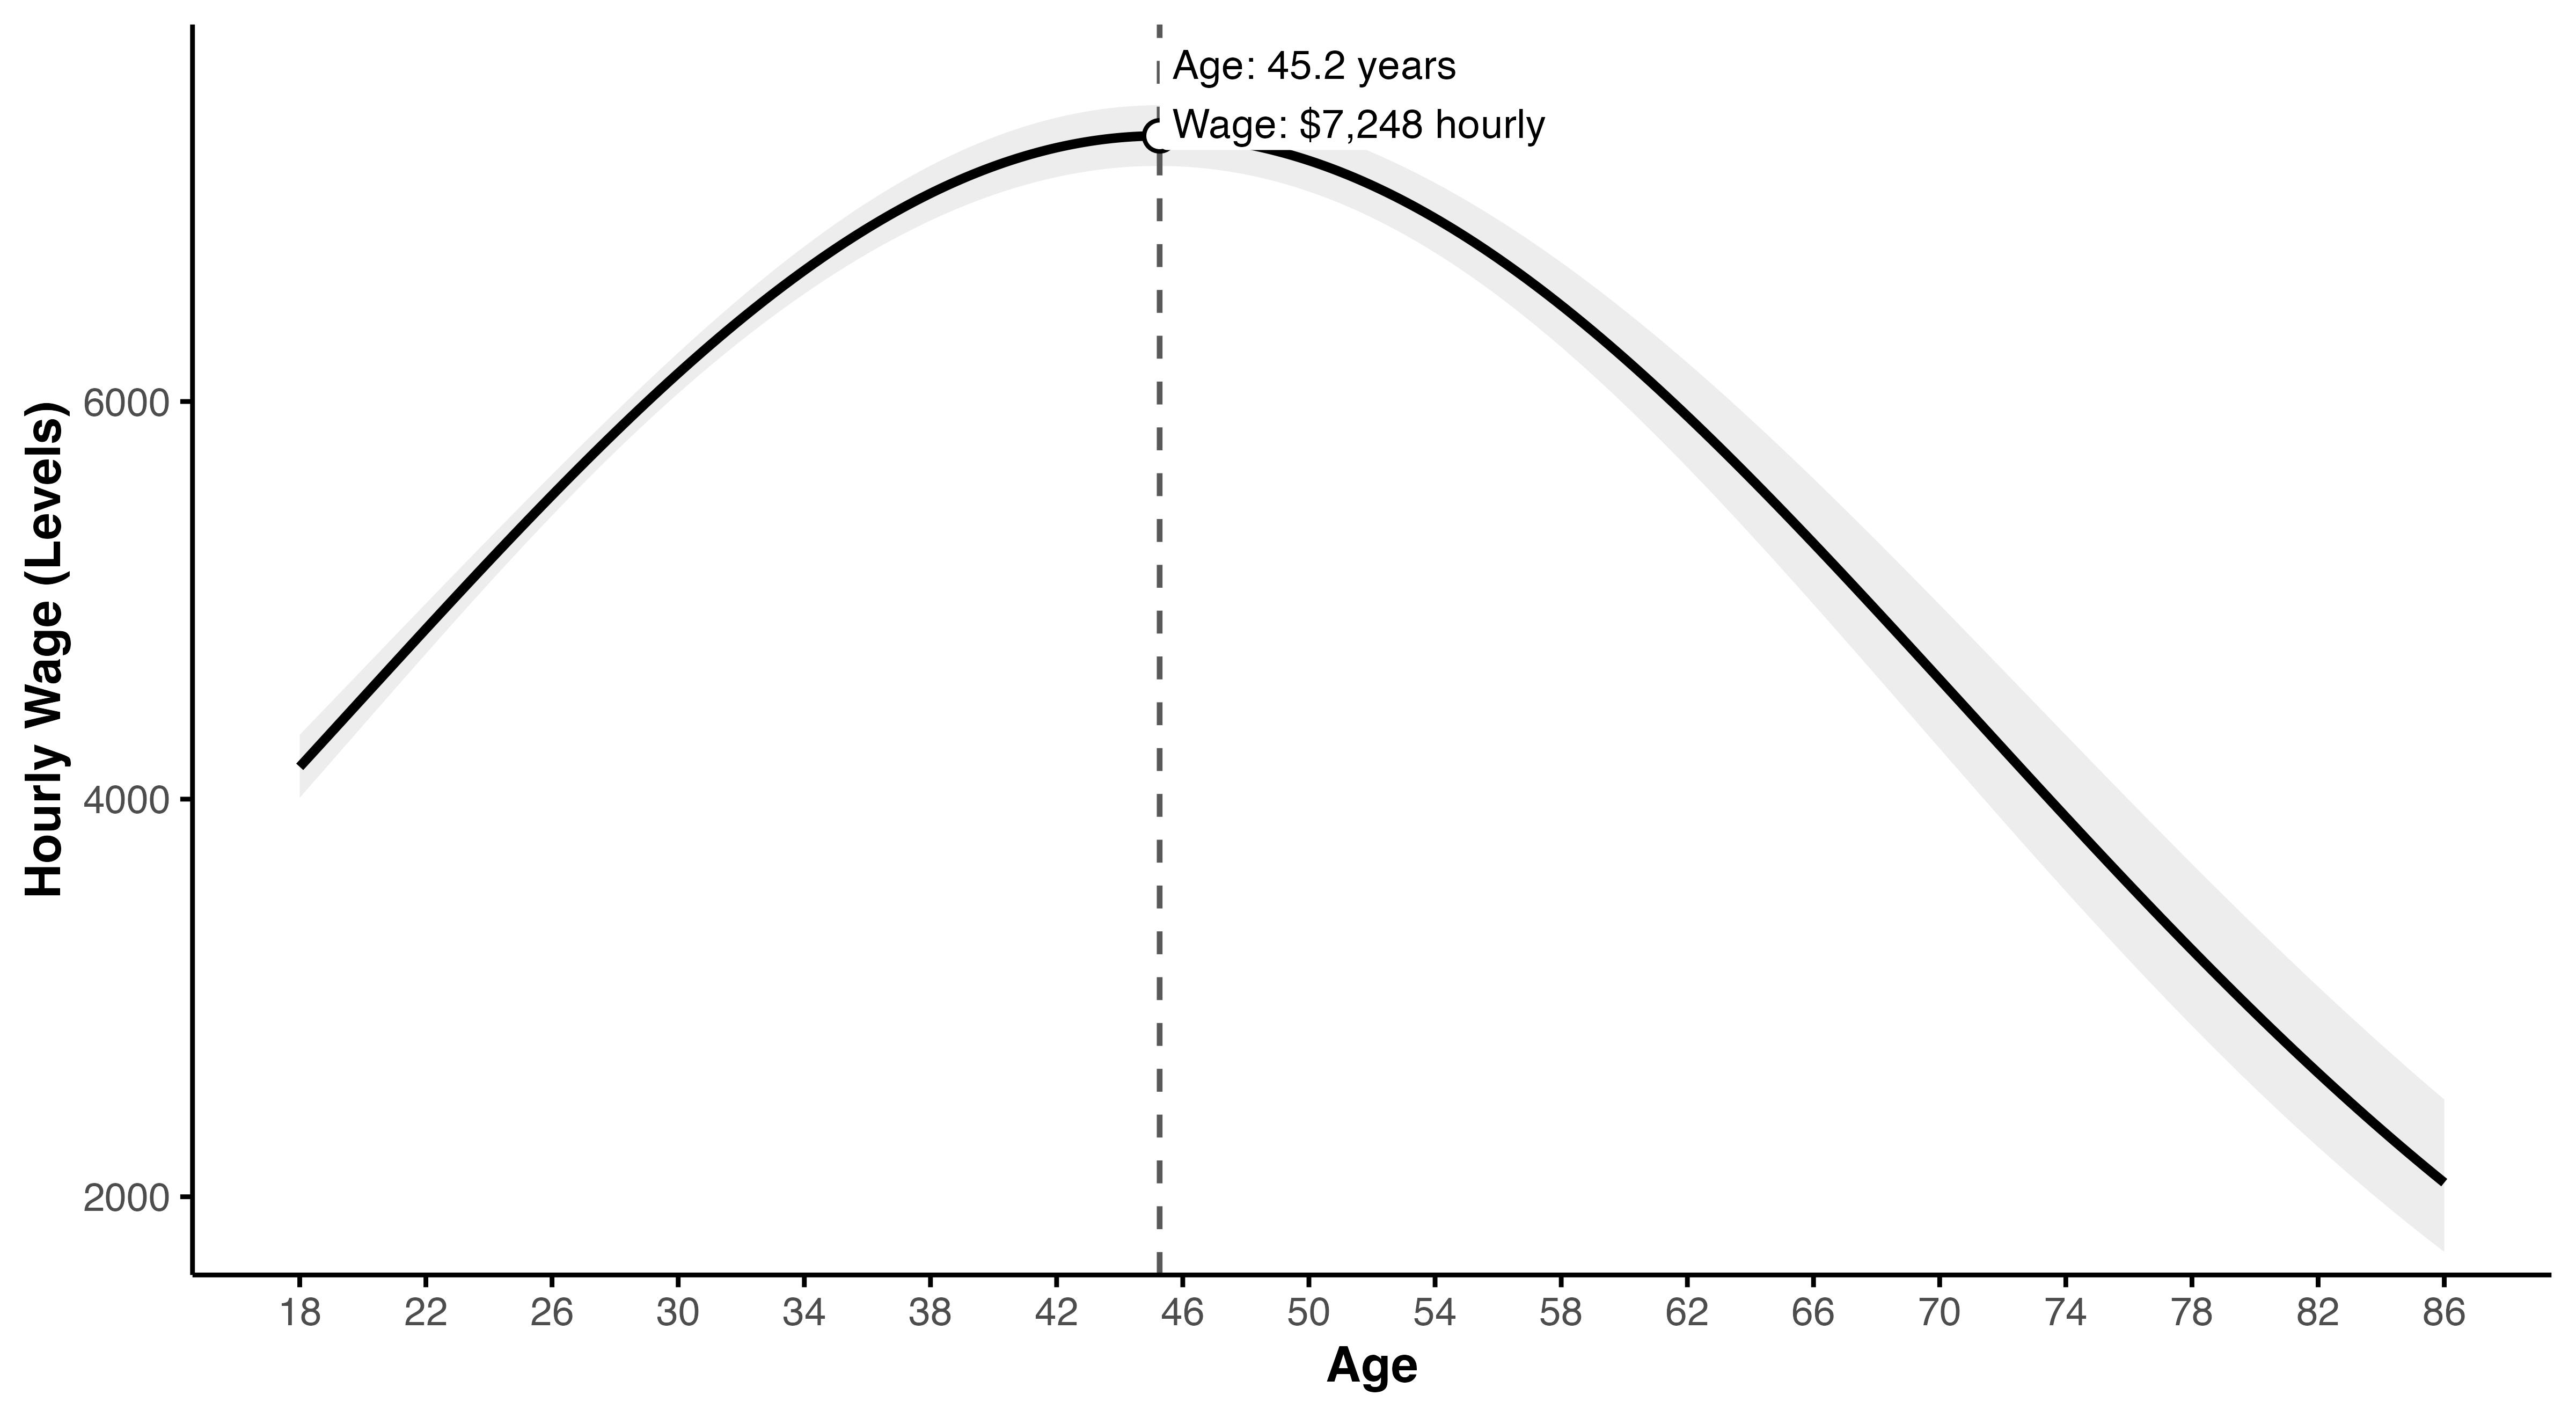
\includegraphics[width=0.82\textwidth]{figures/perfil_edad_salario_base.jpg}

  \caption*{\footnotesize \textit{Notes:} The dashed line marks the peak age; the dot annotates the peak wage.}
\end{center}


\section{The gender earnings GAP}

The gender wage gap has long been a central topic in labor economics, with evidence pointing to persistent disparities that cannot be fully explained by productivity differences alone (Goldin, 2014). To estimate the effect of being female on hourly wages, we rely on the Frisch-Waugh-Lovell (FWL) theorem, which allows us to partial out sets of controls and isolate the residual contribution of gender. \autoref{tab:gendergap} reports our estimates across four specifications, beginning with an unconditional regression and progressively introducing controls for individual characteristics (years of education, age, and age$^2$), firm attributes (formality, sector, and firm size), and occupation. 

\begin{table}[!htbp] \scriptsize\centering 
  \caption{Female-Wage unconditional and conditional regressions.} 
  \label{tab:gendergap} 
\begin{tabular}{@{\extracolsep{5pt}}lcccc} 
\\[-1.8ex]\hline 
\hline \\[-1.8ex] & No Controls & Individual controls & Firm controls & Occupation controls \\ 
\\[-1.8ex] & (1) & (2) & (3) & (4) \\ 
\hline \\[-1.8ex] 
Female (=1) / Residual FWL & $-$0.047$^{***}$ & $-$0.138$^{***}$ & $-$0.105$^{***}$ & $-$0.084$^{*}$ \\ 
 & (0.015) & (0.011) & (0.011) & (0.011) \\ 
Constant & 8.752$^{***}$ & 0.000 & 0.000 & 0.000 \\ 
 & (0.010) & (0.006) & (0.005) & (0.005) \\ 
\hline \\[-1.8ex] 
Controls education/age & No & Yes & Yes & Yes \\ 
Formality, sector and firm size & No & No & Yes & Yes \\ 
Type of occupation & No & No & No & Yes \\ 
Observations & 9,700 & 9,700 & 9,700 & 9,700 \\ 
R$^{2}$ & 0.001 & 0.016 & 0.010 & 0.006 \\ 
Adjusted R$^{2}$ & 0.001 & 0.016 & 0.009 & 0.006 \\ 
Residual Std. Error (df = 9698) & 0.721 & 0.545 & 0.512 & 0.463 \\ 
F Statistic (df = 1; 9698) & 10.270$^{***}$ & 155.092$^{***}$ & 93.887$^{***}$ & 55.306$^{*}$ \\ 
\hline 
\hline \\[-1.8ex] 
\multicolumn{5}{c}{\scriptsize $^{*}$p$<$0.1;\; $^{**}$p$<$0.05;\; $^{***}$p$<$0.01} \\ 
\end{tabular} 
\end{table}

The unconditional regression (1) indicates that women earn on average 4.7 percent less per hour than men, what at first glance may appear as a modest difference. However, when comparing women and men with similar observable characteristics (years of education, age, and age squared), as in specification (2), the gap jumps to 13.8\%. This occurs because, as shown in the descriptive statistics, women in our sample tend to be more educated than men. Thus, failing to account for these differences leads the unconditional estimate to understate the true wage disparity. 

Including firm-level characteristics in (3)-such as whether the job is formal or informal, whether it belongs to the public or private sector, and the size of the firm--reduces the gap to 10.5\%. This reflects the fact that women are more likely to self-select into smaller or less formal firms, which generally pay lower wages. Finally, specification (4) adds controls for occupation, further reducing the gap to 8.4 percent. This highlights that occupational sorting-with women disproportionately concentrated in lower-paying professions-explains part of the observed disparity. 

Using FWL tends to provide wrong standard errors due to the incapacity to recognize the complete set of estimators that were omitted in the final regression, that is why bootstrap is used to recalculate properly this values. Doing so for model 4 (all controls), we can observe a bias of -0.0002, which is really small and shows a good performance of the initial estimation. Also, the confidence intervale is between -10.8\% and -6\% at a 95\% level; validating the statistical significance of the estimator.

Overall, the sequential introduction of controls reveals a combination of selection and discrimination effects. Selection is evident in women's greater representation in smaller, less formal firms and lower-paying occupations. Yet, even after accounting for these compositional differences, a residual gap of 8.4\% percent remains. This indicates that women with comparable education, age, firm characteristics, and professional roles still earn significantly less than men, providing strong evidence against the notion of ``equal pay for equal work.''

\subsection{Gender-Age Gap} 

Additionally, analyzing the age-wage peak separately for each gender could potentially reveal the interaction between two factors: age and gender, which may disproportionately affect older women. This was solved by adding into model 3 interactions between $Age$ and $Age^2$ with $Female$. In \autoref{fig:agecurve2}, we observe that the peak age at which men and women reach their maximum wages is at 62 for women and 65 for men. Prior research suggests that this U-shaped pattern, typically showing a peak in the fifties, largely reflects the cross-sectional nature of wage data. Wages do not necessarily decline at older ages; rather, they tend to remain relatively stable, while the apparent decline is driven by partial retirement and gradual reductions in labor supply among older workers \citep{Luong2009, Casanova2012, Scarfe2023}. A more detailed discussion of why these estimated peaks change substantially once controls are introduced is provided in the Appendix.


% con controles
\begin{center}
\captionsetup{type=figure,position=top}
  \captionof{figure}{Age-Wage Profile by sex: Conditional Estimation.}
  \label{fig:agecurve2}
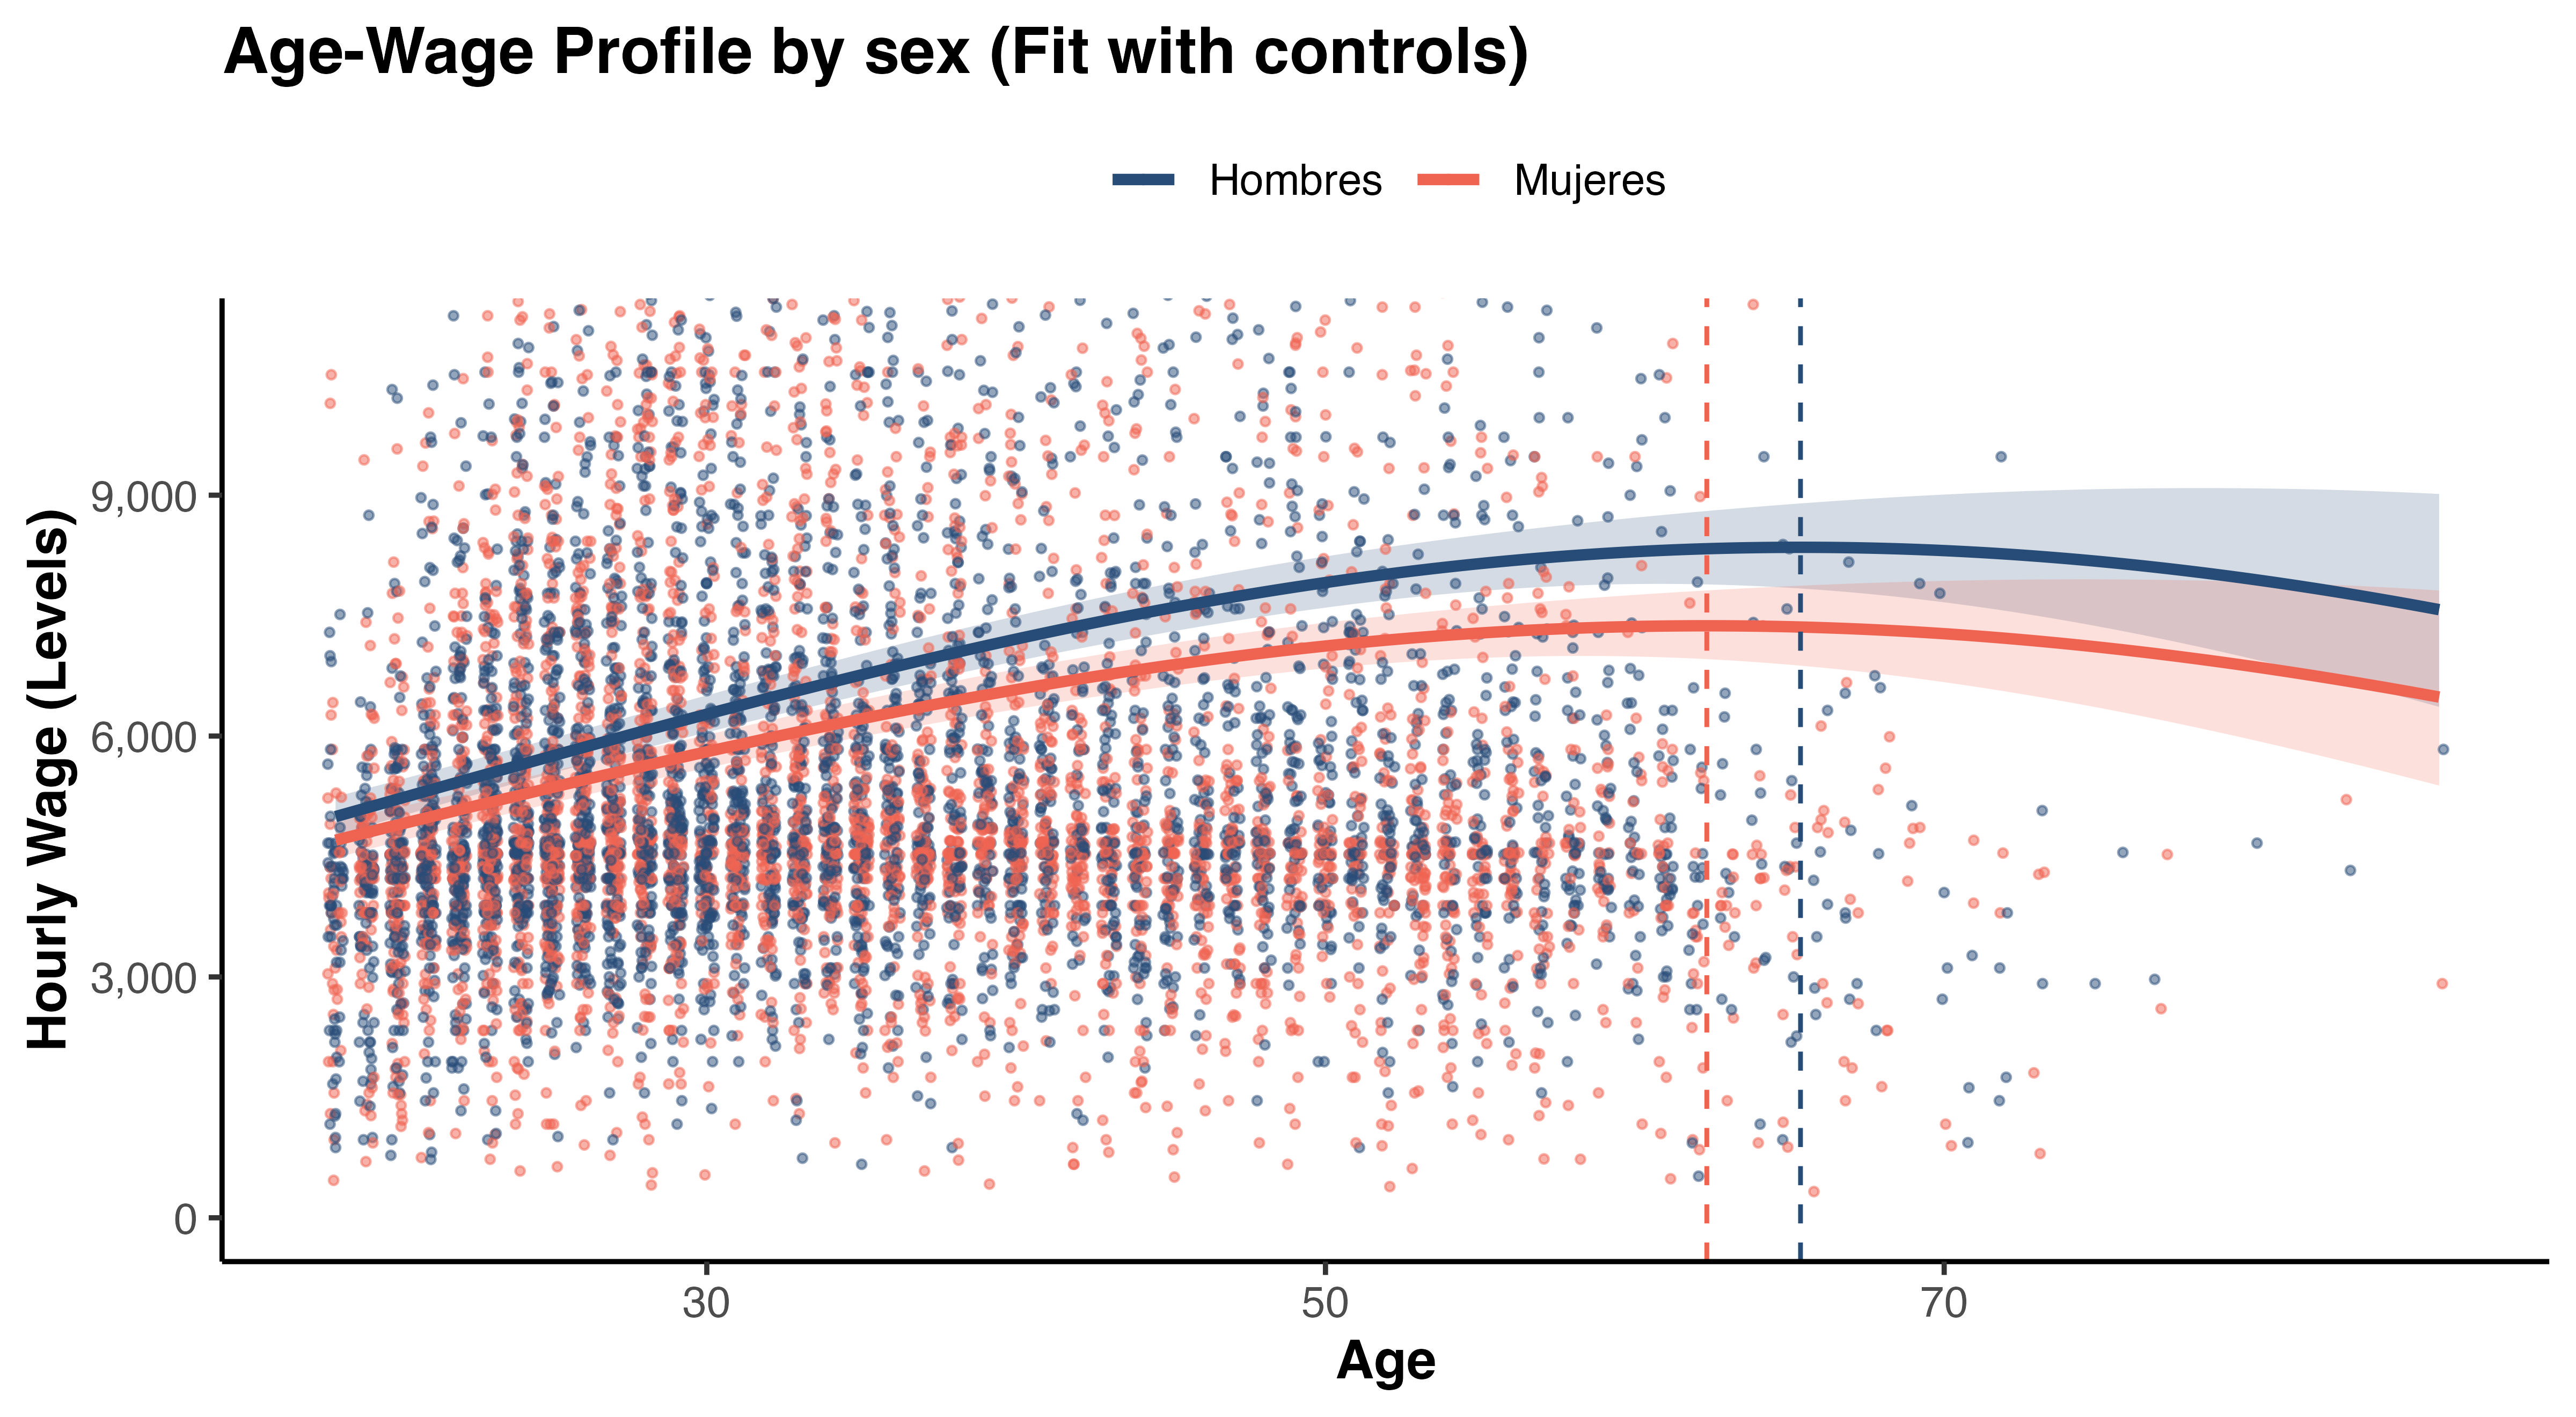
\includegraphics[width=0.8\textwidth]{figures/perfil_edad_salario_controles.jpg}
\label{fig:agecurve2}
\end{center}

The estimated wage-age trajectories for both genders display a similar shape, with the primary difference being the scale of earnings at each age-women reaching a peak salary of \$7,373 per hour, and men \$8,350, almost 14\% less. Statistically speaking, these peaks are not significantly different, as a hypothesis test using the t-Student method yields a p-value of 0.6. This further suggests that, when controlling for the factors discussed earlier, men and women follow similar age-wage patterns; however, gender still influences the overall level of earnings, with men generally earning higher salaries throughout their careers.

\section{Predicting wages}
Now, moving away from the standard econometrical view that only focuses on causality and estimators analysis, we will try to predict the salary per hour using various specifications, including the ones presented before.

\textbf{Validation Set Approach (VS):} Using a sample of 70\% of the total sample (6794 observations) for training and 30\%(2906) for testing, we selected 8 specification to try to predict salary per hour (That will be listed in the appendix).

   \begin{table}[h!]
\caption{RMSE of Predicted Models using Validation Set Approach.}
\label{tab:rmse_vs}
\centering
\renewcommand{\arraystretch}{1.15}
\begin{tabular}{l D{.}{.}{4}}
\toprule
Model & \multicolumn{1}{c}{RMSE VS} \\
\midrule
Additional 2 & 0.4502 \\
Additional 1 & 0.4543 \\
Base 2       & 0.4706 \\
Additional 4 & 0.4713 \\
Additional 5 & 0.5372 \\
Additional 3 & 0.5405 \\
Base 0       & 0.7069 \\
Base 1       & 0.7230 \\
\bottomrule
\end{tabular}
\end{table}

In \autoref{tab:rmse_vs}, we observe the Root Mean Square Error (RMSE) of the specifications listed in the appendix (, organized from the lowest to the highest. Overall we can see that, besides Model Base 0 and 1, the models have a good perfomance calculating the LogHourlyWage. Calculating the relative error in percentage, by evaluating each RMSE with $e$ and subtracting $-1$, we can observe that the first 6 models predictions are around 56\% and 70\% difference of the original value, and the last two, around 100\%.
Model Additional 2 showed the lowest RMSE with 0.4502. This specification is an improvement compared to the conditional gender earnings gap presented in  previous sections intended to increase its predicting potential. Specifically, this model adds variables such as Age to the 3 and 4 for more complexity and non-linearity and also the socioeconomical status, a variables that while predicting the gaps in gender might be as relevant as other persona characteristics, for predicting the wages is really crucial since it classifies people into categories for economical status depending on where you live. 

To identify the observations that ``missed the mark", we defined these as those points that were more than 2 standard deviations away from the mean; a total of 167 observations ``missed the mark" in the prediction.

\begin{table}[!htbp] \centering \scriptsize
  \caption{Observations that "missed the mark" main characteristics} 
  \label{tab:missedthemark} 
\begin{tabular}{@{\extracolsep{5pt}}lccccc} 
\\[-1.8ex]\hline 
\hline \\[-1.8ex] 
Statistic & \multicolumn{1}{c}{N} & \multicolumn{1}{c}{Mean} & \multicolumn{1}{c}{St. Dev.} & \multicolumn{1}{c}{Min} & \multicolumn{1}{c}{Max} \\ 
\hline \\[-1.8ex] 
Monthly Wage& 167 & 5,227,224.000 & 7,907,487.000 & 60,000.000 & 60,100,000.000 \\ 
Total Hours Worked & 167 & 45.826 & 14.212 & 10 & 84 \\ 
Age & 167 & 38.108 & 12.973 & 18 & 71 \\ 
Male & 167 & 0.515 & 0.501 & 0 & 1 \\ 
Socialeconomical Status & 167 & 3.084 & 1.333 & 1 & 6 \\ 
Years of Education & 167 & 13.862 & 4.362 & 0 & 22 \\ 
Experience & 167 & 18.246 & 13.996 & 0 & 60 \\ 
\hline \\[-1.8ex] 
\end{tabular} 
\end{table} 


In \autoref{tab:missedthemark} we can observe the main characteristics of these 167 observations in the most relevant variables in our dataset. Overall, we can not identify clear patterns in variables such as Age, Male, Socialeconomical Status, Years of education or Experience, since they are well between the same distributions of all the observations as showed during previos sections. Nonetheless it is important to identify the behaviour of Monthly Wage to see any patterns regarding the Salary.\\

\begin{center}
  \captionsetup{type=figure,position=top}
  \captionof{figure}{Laboral Wage of Prediction Error Outliers}
  \label{fig:agecurve3}

  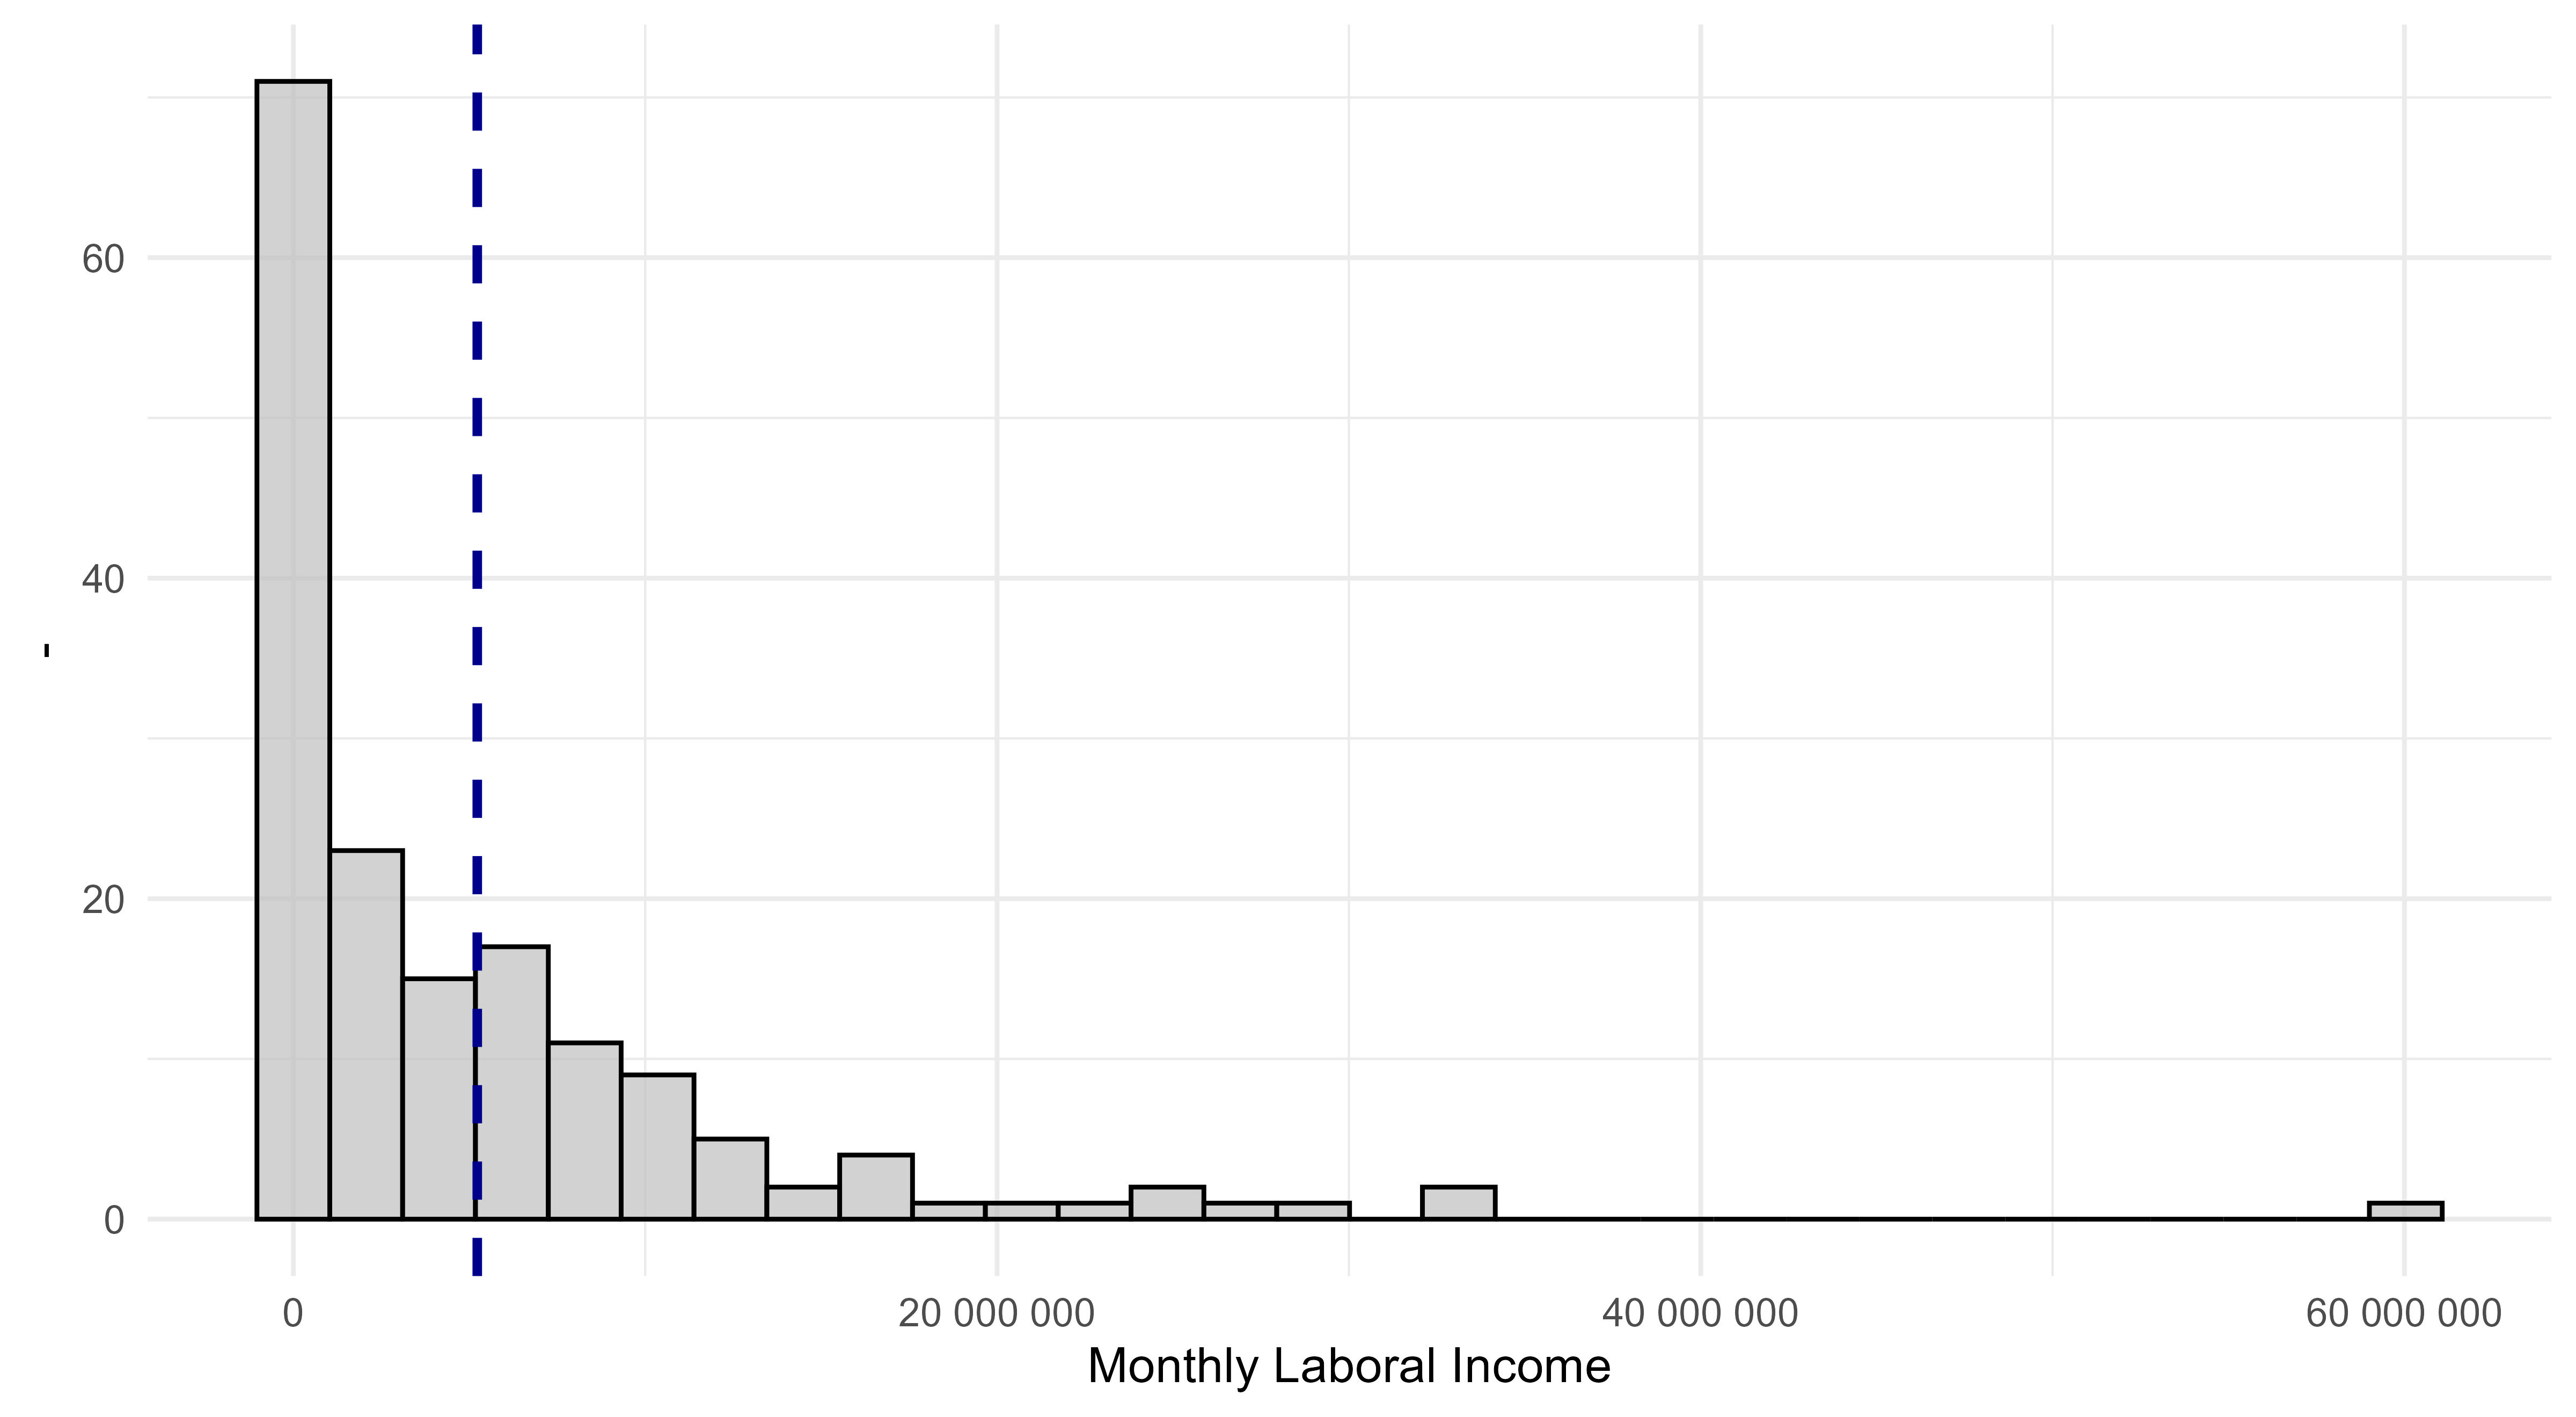
\includegraphics[width=0.7\textwidth]{figures/G5outliers.jpg}
\end{center}

  Figure 3 shows that most of the observation presenting prediction errors tend to be allocated in the left wing of the distribution, reporting less than \$5000000 in Monthly Laboral Wage. It is important to note that, when most of the distributions is around the same values, the fact that this predictions miss the values in such a significant way, raise an alarm to look into the values reported, to avoid any kind of under reporting for tax evation.
  
\textbf{LOOCV.} For the top 2 specifications with the lowest RMSE, resampling methods such as K-fold Cross-Validation (K-fold CV) and Leave One Out Cross-Validation (LOOCV) were used to validate the initial prediction value and to identify if these RMSE are consistent and the models do capture a good prediction or if we are over-fitting the models, making them good for that specific partition but not as good for any other kind of sample. For the case of K-fold Cross-Validation, k=10 was used, as is standard within the discipline. This was done to verify whether the use of a more computationally lightweight model yields results that do not differ significantly or, alternatively, to analyze potential influential observations that might be biasing the results in certain partitions.

\begin{table}[h!]
\caption{RMSE of Predicted Models using Validation Set Approach, K-fold CV, and LOOCV}
\label{tab:rmse_vsloocv}
\centering
\renewcommand{\arraystretch}{1.15}
\begin{tabular}{l c c c}
\toprule
Model & RMSE\_VS & RMSE\_K-fold CV & RMSE\_LOOCV \\
\midrule
Additional 2& 0.4502 & 0.4486 & 0.4493 \\
Additional 1 & 0.4543 & 0.4543 & 0.4533 \\
\bottomrule
\end{tabular}
\end{table}

In \autoref{tab:rmse_vsloocv}, we present the RMSE results from K-fold CV and LOOCV, compared to the original RMSE obtained from the validation set (VS) approach. We observe that the predictions from the VS approach are consistent with those from the more sophisticated training-testing methods. If the results had shown significant differences between VS and the other approaches, it might suggest that some influential observations were impacting the prediction model within the specific partition used in the first approach. This would warrant an investigation into why these observations have such an effect on the model’s predictions and whether their inclusion or exclusion is beneficial for the overall training process.



\bibliography{References}

%apaendice 1
\section{Appendix}

\subsection{ Specifications for prediction in "Predicting Wages"}

\begingroup
\small
% Espaciado de displays solo en este bloque (compacto)
\setlength{\abovedisplayskip}{4pt}
\setlength{\belowdisplayskip}{4pt}
\setlength{\abovedisplayjot}{}
\setlength{\jot}{2pt}

\begin{description}[style=nextline, leftmargin=0pt, labelwidth=0pt, labelsep=0pt, itemsep=2pt, topsep=2pt]

\item \textbf{Base 0:}
\[
\text{Log Hourly Wage}_i
  = \beta_0 + \beta_1\,\text{Age}_i + \beta_2\,(\text{Age}_i)^{2} + \varepsilon_i
\]

\item \textbf{Base 1:}
\[
\text{Log Hourly Wage}_i
  = \beta_0 + \beta_1\,\text{Female}_i + \varepsilon_i
\]

\item \textbf{Base 2:}
\[
\begin{aligned}
\text{Log Hourly Wage}_i
  &= \beta_0 + \beta_1\,\text{Female}_i + \beta_2\,\text{Years of Education}_i \\
  &\quad + \beta_3\,\text{Age}_i + \beta_4\,(\text{Age}_i)^{2} \\
  &\quad + \beta_5\,\text{Formal Business}_i + \beta_6\,\text{Size Firm}_i \\
  &\quad + \beta_7\,\text{Laboral Relation}_i + \beta_8\,\text{Profession}_i + \varepsilon_i
\end{aligned}
\]

\item \textbf{Additional 1:}
\[
\begin{aligned}
\text{Log Hourly Wage}_i
  &= \beta_0 + \beta_1\,\text{Female}_i + \beta_2\,\text{Max Educational Year}_i \\
  &\quad + \beta_3\,\text{Experience}_i + \beta_4\,(\text{Experience}_i)^{2} \\
  &\quad + \beta_5\,\text{Formal Business}_i + \beta_6\,\text{Size Firm}_i \\
  &\quad + \beta_7\,\text{Laboral Relation}_i + \beta_8\,\text{Profession}_i + \varepsilon_i
\end{aligned}
\]

\item \textbf{Additional 2:}
\[
\begin{aligned}
\text{Log Hourly Wage}_i
  &= \beta_0 + \beta_1\,\text{Female}_i + \beta_2\,\text{Years of Education}_i \\
  &\quad + \beta_3\,\text{Age}_i + \beta_4\,(\text{Age}_i)^{2} \\
  &\quad + \beta_5\,(\text{Age}_i)^{3} + \beta_6\,(\text{Age}_i)^{4} \\
  &\quad + \beta_7\,\text{Formal Business}_i + \beta_8\,\text{Size Firm}_i \\
  &\quad + \beta_9\,\text{Laboral Relation}_i + \beta_{10}\,\text{Profession}_i \\
  &\quad + \beta_{11}\,\text{Socioeconomical Status}_i + \varepsilon_i
\end{aligned}
\]

\item \textbf{Additional 3:}
\[
\begin{aligned}
\text{Log Hourly Wage}_i
  &= \beta_0 + \beta_1\,\text{Female}_i + \beta_2\,\text{Years of Education}_i \\
  &\quad + \beta_3\,\text{Age}_i + \beta_4\,(\text{Age}_i)^{2} \\
  &\quad + \beta_5\,(\text{Age}_i \times \text{Female}_i) \\
  &\quad + \beta_6\,(\text{Age}_i^{2} \times \text{Female}_i) \\
  &\quad + \beta_7\,(\text{Age}_i \times \text{Years of Education}_i) + \varepsilon_i
\end{aligned}
\]

\item \textbf{Additional 4:}
\[
\begin{aligned}
\text{Log Hourly Wage}_i
  &= \beta_0 + \beta_1\,\text{Female}_i + \beta_2\,\text{Years of Education}_i \\
  &\quad + \beta_3\,\text{Age}_i + \beta_4\,(\text{Age}_i)^{2} \\
  &\quad + \beta_5\,(\text{Age}_i)^{3} + \beta_6\,(\text{Age}_i)^{4} \\
  &\quad + \beta_7\,\text{Experience}_i + \beta_8\,(\text{Experience}_i)^{2} \\
  &\quad + \beta_9\,(\text{Experience}_i)^{3} + \beta_{10}\,(\text{Experience}_i)^{4} \\
  &\quad + \beta_{11}\,(\text{Experience}_i)^{5} \\
  &\quad + \beta_{12}\,\text{Formal Business}_i + \beta_{13}\,\text{Size Firm}_i \\
  &\quad + \beta_{14}\,\text{Laboral Relation}_i + \beta_{15}\,\text{Profession}_i \\
  &\quad + \beta_{16}\,\text{Socioeconomical Status}_i + \beta_{17}\,\text{College}_i \\
  &\quad + \beta_{18}\,(\text{Age}_i \times \text{Female}_i) \\
  &\quad + \beta_{19}\,(\text{Age}_i^{2} \times \text{Female}_i) + \varepsilon_i
\end{aligned}
\]

\item \textbf{Additional 5:}
\[
\begin{aligned}
\text{Log Hourly Wage}_i
  &= \beta_0 + \beta_1\,\text{Experience}_i + \beta_2\,(\text{Experience}_i)^{2} \\
  &\quad + \beta_3\,(\text{Experience}_i)^{3} + \beta_4\,(\text{Experience}_i)^{4} \\
  &\quad + \beta_5\,(\text{Experience}_i)^{5} + \beta_6\,(\text{Experience}_i)^{6} \\
  &\quad + \beta_7\,(\text{Experience}_i)^{7} + \beta_8\,\text{Profession}_i \\
  &\quad + \beta_9\,(\text{Profession}_i \times \text{Experience}_i) + \varepsilon_i
\end{aligned}
\]

\end{description}
\endgroup
\subsection{Age-Wage Profile - an Unconditional Estimation}

Additionally, we wanted to present how the peak ages would change in the initial unconditional model for Gender Earnings Gap.

This results reflect the condition of the gap before controlling the observations and identifying the possible mix effect described in the main body of the paper.



\begin{center}
  \captionsetup{type=figure,position=top}
  \captionof{figure}{Age-Wage Profile by sex: Unconditional Estimation}
  \label{fig:agecurve3}

  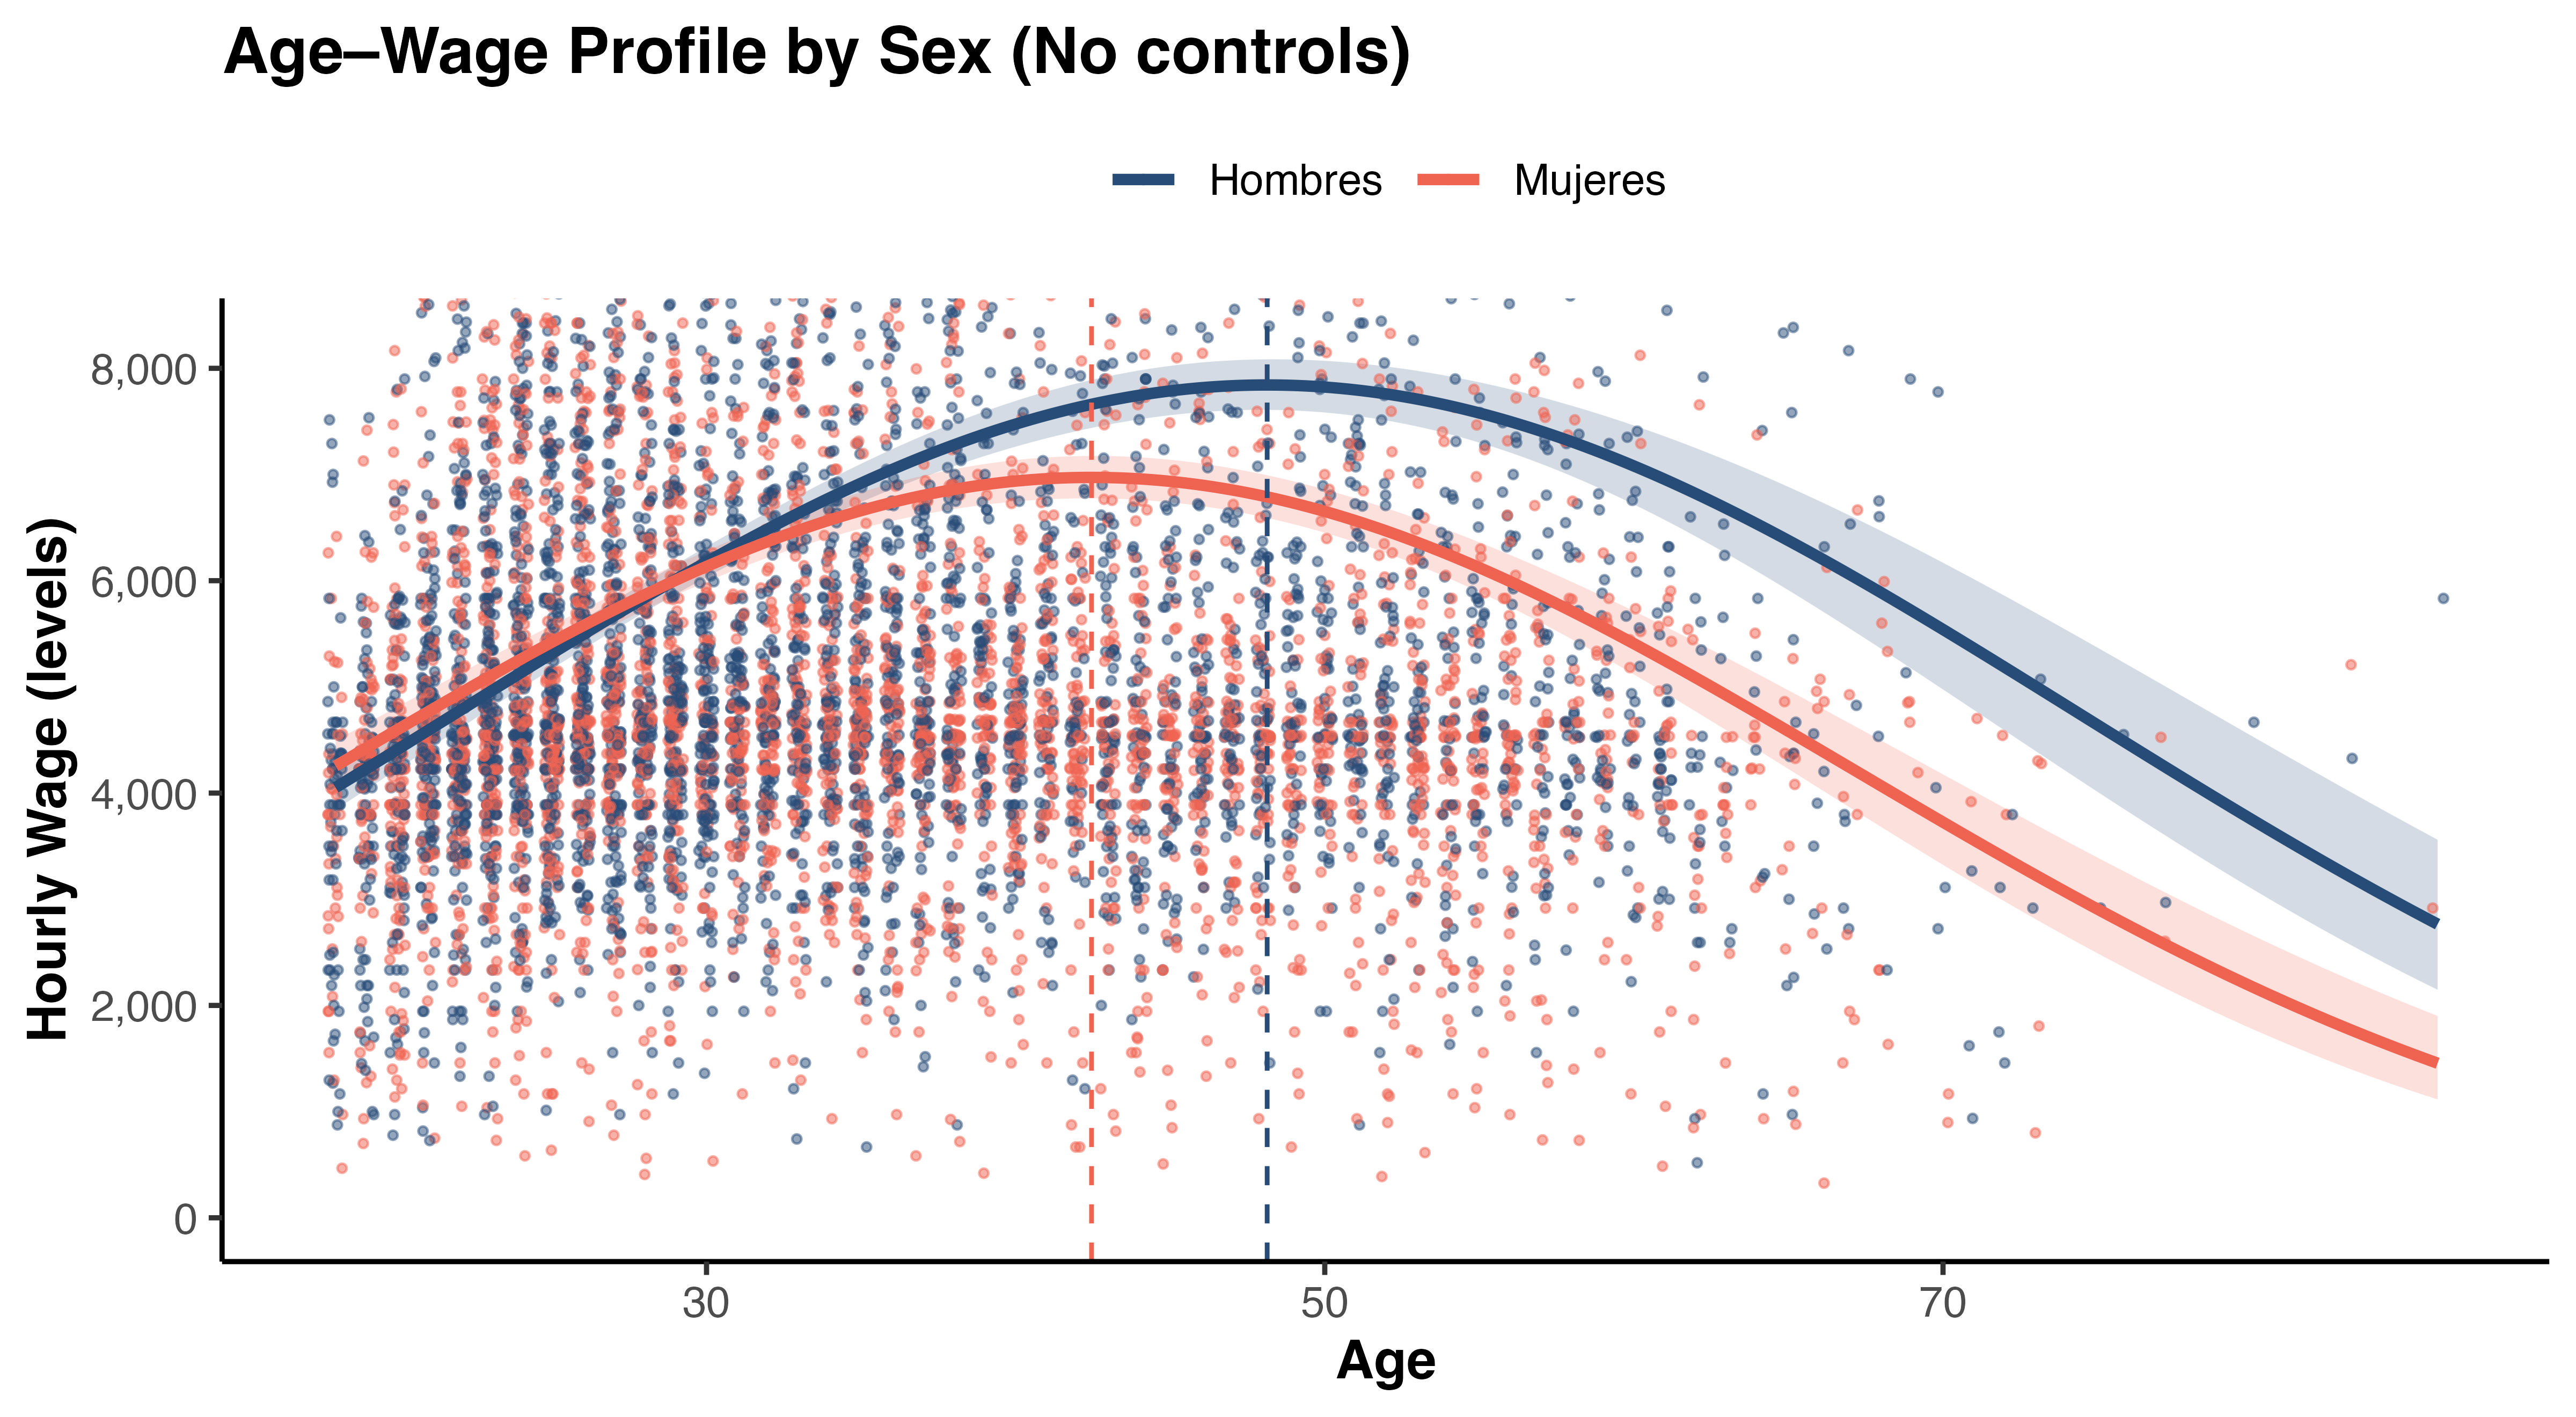
\includegraphics[width=0.8\textwidth]{figures/perfil_edad_salario_nocontroles.jpg}
\end{center}

In figure 4 we can observe how men and women tend to have equal salaries, but then women start to fall behind, which is consistent with the estimation of model 2 in the gender age gap that included individual characteristics; women tend to be underpaid, in reference to men, when taking into account age characteristics, with this indication that around 40 years old, the divergence between the two gender starts.

Lastly, this unconditional version, speaks directly to the Figure 1, since having an almost perfectly distributed sample in gender (~ 50\% women and 50\% men) could allow us to average the two peaks (48.1 for men and 42.4 for women) and find the same peak age for all the sample, 45.2)

\end{document}

